\subsection{\raspi}\label{sec:raspi}
Der Raspberry Pi 4\autocite{Raspberry} ist ein leistungsstarker Einplatinencomputer, der über einen Quad-Core ARM Cortex-A72 Prozessor mit Geschwindigkeiten von bis zu 1,5 GHz und bis zu 8 GB LPDDR4 RAM verfügt. Der Raspberry Pi 4 bietet verbesserte Grafikfähigkeiten dank eines Broadcom VideoCore VI Grafikprozessors und unterstützt 4K-Video bei 60 Bildern pro Sekunde über HDMI. Mit Gigabit-Ethernet, WLAN, Bluetooth, USB 3.0 und USB-C-Stromversorgung bietet er eine Vielzahl von Konnektivitätsoptionen. Der Raspberry Pi 4 verfügt auch über GPIO-Pins für die Interaktion mit elektronischen Komponenten und Sensoren. Dank seiner Kompatibilität mit verschiedenen Betriebssystemen und der Unterstützung einer engagierten Community eignet sich der Raspberry Pi 4 für eine Vielzahl von Anwendungen, von Heimautomatisierung bis hin zur Entwicklung von IoT-Geräten und als preiswerte Desktop-Alternative.\\
\vspace{5mm}
Der Raspberry Pi ist perfekt für unsere DA geeignet, da er sowohl über Ein- als auch Ausgänge verfügt und sich ideal für die Steuerung über eine Website eignet. Die GPIO-Pins ermöglichen es uns, mit verschiedenen Sensoren, Aktoren und anderen externen Geräten zu interagieren, während gleichzeitig die Möglichkeit besteht, die Steuerung und Überwachung über eine Webanwendung zu realisieren. Diese Kombination aus physischer Einbindung und webbasierter Steuerung bietet die Flexibilität und Leistungsfähigkeit, die wir für die Umsetzung unserer DA benötigen.
\vspace{5mm}
\begin{figure}[H]
    \centering
    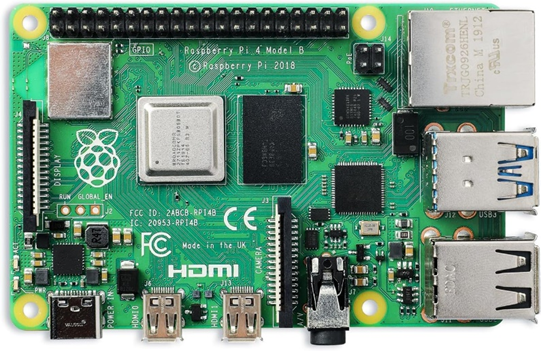
\includegraphics[scale=0.8]{image/raspi.png}
    \caption{\raspi}
    \label{fig:enter-label}
\end{figure}